\documentclass[12pt]{extreport}

\usepackage[a4paper, total={6in, 8in}]{geometry}
\usepackage{amsfonts}
\usepackage{amsmath}
\usepackage{amsthm}
\usepackage{hyperref}
\usepackage{tikz}
\usepackage{graphicx}
\usepackage{float}
\usepackage[utf8]{inputenc}
\usepackage{fontenc}
\usepackage[boxruled,linesnumbered]{algorithm2e}
\usepackage{booktabs}
\usepackage{multirow}
\usepackage{adjustbox}
\usepackage{cleveref}
\usepackage[sorting=none, backend=biber]{biblatex}
\usepackage{svg}

%For fun only...
\usepackage{times}

%Bibliographies
\bibliography{references,rfc}

\theoremstyle{plain}
\newtheorem{theorem}{Theorem}[section]
\newtheorem{lemma}[theorem]{Lemma}
\newtheorem{proposition}[theorem]{Proposition}
\newtheorem*{corollary}{Corollary}

\theoremstyle{definition}
\newtheorem{definition}{Definition}[section]
\newtheorem{conjecture}{Conjecture}[section]
\newtheorem{example}{Example}[section]

\theoremstyle{remark}
\newtheorem*{remark}{Remark}
\newtheorem*{note}{Note}

\crefname{algocf}{alg.}{algs.}
\Crefname{algocf}{Algorithm}{Algorithms}

%Title
\title{Some Security Considerations over Contiki-based Sensor Network}
%Authors
\author{Yan Yan}
\date{\today}

\begin{document}

\maketitle

\tableofcontents

%Body
%%\chapter{Some Chapter}

\section{Some Section}

Contents\cite{SomeCitation}...

\section{Introduction}
Applications for the Internet of Things (IoT) flourish, leaving a great desire for not only energy efficient, cheap devices, but also for devices that support basic cryptographic functionality such as confidentiality and/or authenticity. Popular algorithms for confidentiality are e.g. the Advanced Encryption Standard\cite{AES}, and the Elliptic Curve Digital Signature Algorithm\cite{ECDSA}, which, when used in conjunction, enable to establish secure end-to-end channels via e.g. Datagram TLS\cite{DTLS}. 

However whilst AES is a secure block cipher, one might require randomness to turn it into a secure encryption scheme for arbitrary length messages. Somewhat similarly, ECDSA relies on a known-to-be-secure mathematical problem. However, it also requires large and securely generated random numbers. Consequently, when supporting cryptography the secure generation of random numbers is crucial. 

%The prospering IoT applications constantly proposes higher requirements to security where cryptography plays an important role. Among all prerequisite of implementing cryptographic primitives on these IoT devices, a reliable Random Number Generator (RNG) is critical as it is required in most cryptographic algorithms. In practice, a RNG typically involves a Pseudo Random Number Generator (PRNG) seeded by a high entropy physical source.

In 2013, Texas Instruments (TI) launched a new System-on-chip (SoC), the CC2538\cite{CC2538}, featuring secure channels via 802.15.4\cite{802154Standard} support via multiple cryptographic hardware accelerators. Partially because this cryptographic accelerators, projects such as Contiki\cite{Contiki} and OpenWSN\cite{OpenWSN} began to support the CC2538 with enthusiasm. As of writing this paper, the chip features in the suggested list for Zigbee and 6LoWPAN solution on TI's website\cite{ZigbeeProducts}\cite{6LowPANProducts}.

However, despite all the cryptographic hardware support, the CC2538 does not have a RNG dedicated for cryptographic applications; instead, the user manual suggests to use a 16 bit Linear Feedback Shift Register (LFSR) as a PRNG where the seed is generated by the Radio Frequency (RF) module sampling from the radio noise. Whilst the user guide at no point suggests that this method should be used in conjunction with cryptographic algorithms, developers have little choice in the absence of alternatives. Also, in the absence of published attacks, there is often a temptation to ignore warnings such as in \cite{SmartMeterBlog}. 

\subsection{Our Contribution}
We show in this study that this choice proves catastrophic for cryptographic applications, not only because the in-built PRNG has only 16 bit entropy which can be easily predicted, but also because we are able to practically demonstrate how to use radio jamming to bias the seed obtained from the RF module. Consequently, even if the weak in-built PRNG was replaced by a stronger component, the source for the seed could still be tampered with and thus render the system insecure. All the experimental work in this paper was performed on Contiki OS\cite{Contiki} release version 3.0. 
%The related source code can be accessed at \cite{prngtest}.

Our paper is structured as follows. We begin in \Cref{ContikiDriverIssue} with some Contiki RNG driver issues for CC2538. \Cref{LFSR} revises why using a 16 bit LFSR as PRNG is a bad practice and we show how this design flaw can be exploited to break DTLS in \Cref{BreakDTLS}, before reviewing the problem in \Cref{PRNGReflection}. In \Cref{Seed} we explain how CC2538 samples the radio noise into random seed and then we demonstrate how it can be biased by jamming signals in \Cref{Jamming}. Finally we conclude the paper in \Cref{Conclusion}.

\subsection{Related Work}
The design flaw of using a 16 bit LFSR as PRNG has been reported by \cite{SmartMeterBlog}\cite{CC2530PRNG} on CC2430\cite{CC2430Manual} and CC2530\cite{CC2530Manual} respectively. These chips are the predecessors of CC2538 in the SimpleLink\cite{SimpleLink} series and they all adopted the same RNG design. The blogs reported the flaw and warned that it could easily be exploited to break the Z-Stack library\cite{ZStack} and Smart Energy Profile ECC in many Smart Meter applications. We essentially `rediscovered' that this poor design choice still features in the CC2538 product. However, whilst in previous work the possibility of injecting a jamming signal was contemplated, we are the first to actually examine the technical feasibility of this and to demonstrate a working attack.


\subsection{Contiki Driver Issues}\label{ContikiDriverIssue}
We made extensive use of Contiki in our research and fixed (and reported) some coding issues in their RNG driver (release-3.0). These were, the reading out of the LFSR without ready check, a lack of validity check when reading random seed bits from the RF module, and a bug that drops the Most Significant Bit (MSB) and leaves the Least Significant Bit (LSB) to be constantly zero in the seed.  We modified the code and fixed these issues in our experiments. 

Another issue in the driver is that the CC2538 User's Guide\cite{CC2538Manual} suggests only to use the lower byte (8 bits) as a random number but the driver actually used 16 bits in the LFSR. However, this coding mistake does not affect our result, as will be explained in  later sections.
\chapter{Literature Review} \label{Chp: LiteratureReview}

In this chapter, we will start by introducing the building components of WSN, mainly focuses on different protocol options at each layer. Then we move to security related work, in three aspects of traffic analysis attacks against different Internet applications, attacks against certain protocols and methods for detecting information leakage in different scenarios. Finally we conclude the chapter by cross referencing those  attacks on Internet to the observable metadata in WSN, proposing the potential traffic features that may lead to information leakage.

\section{Building Blocks of WSN}
In this section we categorise the components of WSN by OSI model\cite{OSI}.

The OSI model is a classic model in describing the communication between computing systems (\Cref{fig: OSI model}). The data channel is constructed layer by layer, from the physical medium at the bottom to the abstracted application at the top. Each layer serves a specific purpose, from how to transmit a bit between two physically connected devices to how applications interprets the data.



Before the application data is being sent over the wire, two ends of the communication must agree on protocols being used at each layer. The data is then encapsulated from top layer down to the bottom, as depicted in \Cref{fig: OSI channel}. Each encapsulation adds additional metadata, namely protocol headers, to the data. The process is unwound at the receiving side. Normally lower layer protocols are transparent to upper layers.The outputted encapsulated data from upper layer is simply treated as the payload to a lower layer protocol.

In many cases the boundaries between top three layers are ambiguous; thus they are all referred as Application Layer for convenience.

\begin{figure*}
\centering
{
	\includegraphics[width=0.4\textwidth,]{fig/Osi-model-jb.png}
}
\caption{OSI model} \label{fig: OSI model}
\end{figure*}

\begin{figure*}
\centering
{
	\includegraphics[width=0.6\textwidth,]{fig/Osi-model.png}
}
\caption{Data Transfer in OSI model} \label{fig: OSI channel}
\end{figure*}

\subsection{Physical Layer}
Physical Layer specifies the hardware requirements for devices. It defines data transmission at bit level.

WSN features, as explained by its name, wireless connectivity. 802.15.4\cite{802154} standard is supported in many recent WSN devices. Its Physical Layer specification is intended to be for embedded devices emphasising low energy, low cost and low speed. Bluetooth Low Energy, BLE, is another candidate for WSN with similar features. \cite{802154BLE} provides a performance analysis of 802.15.4 and BLE.

\subsection{Data Link Layer}
Data Link Layer solves the problem of how the media is controlled. It also defines the atomic data chunk, called frames, being transmitted over the physical channel. Data Link protocols are strongly related to physical features of underlining devices. This layer is sometimes referred as MAC layer and the frame is called MAC frame in many context.

With respect to Media Access Control, MAC, technologies such as CSMA/CA \cite{802154} standard and TSCH\cite{TSCH} provides solutions to at which timing and channel should the radio transceiver send and receive data. ContikiMAC\cite{ContikiMAC} proposes a Radio Duty Cycle, RDC, protocol that aims to be energy efficient and has been implemented on Contiki OS.

Another major component in Data Link Layer protocols is the format of different types of frames. In this research, We are particularly interested in its data frame. \Cref{Tbl: 802154 frame} describes the format of a 802.15.4 data frame.

\begin{table}[]
\centering
\begin{tabular}{|c|c|c|c|c|}
\hline
\multicolumn{3}{|c|}{MAC Header}                           & MAC Payload & MAC Footer     \\ \hline
2 (bytes)     & 1                    & 4 to 20              & *           & 2              \\ \hline
Frame Control & Data Sequence Number & Address Information & Data        & Frame Checksum \\ \hline
\end{tabular}
\caption{802.15.4 Data Frame}
\label{Tbl: 802154 frame}
\end{table}

\begin{description}[style=nextline]
\item[\textbf{Frame Control}]
This 2 bytes field contains the bit flags of additional information that instructs how the receiver should interpret this frame, including the type of this frame, whether the security option is enabled and how the source and destination addresses are represented. When the security option is enabled, additional field will be added to the frame. We will explain the security enabled frame format later this section.

\item[\textbf{Data Sequence Number}]
Each packet is assigned a sequence number. The main purpose of this field is that it enables a simple acknowledgement mechanism, ACK, at MAC layer. Since MAC layer provides only unreliable transmission, i.e. MAC frames are allowed to be dropped or arrive disordered; hence the ACK is optional. However, some other protocol can utilise this ACK, e.g. ContikiMAC uses an ACK MAC frame to inform the sender that the frame is received and hence terminates the resending process of sender.

\item[\textbf{Address Information}]
This field contains the source address and destination address of this frame. The length of address is variable. Simply speaking, a longer addresses is used for larger network. and shorter for smaller. Each device has a unique built in address as known as MAC address. The MAC address is configurable on some, in fact nearly all recently, devices. Broadcast is achieved by using a specific destination address but group multicast is not implemented on this layer. In fact, given the physical character of radio, both broadcast messages and unicast messages are technically broadcasted. It entirely depends on the receiver to dropping frames that specifies an unicast address of other nodes.

\item[\textbf{Data}]

\item[\textbf[Frame Checksum]
This is 

\end{description}

\subsection{Network Layer}

\subsection{Transport Layer}

\subsection{Application Layer}

%\cite{802154Sec} discusses some security concerns in 802.15.4.  LLSEC\cite{LLSEC} is the implementation of 802.15.4 security in Contiki.
%
%tinydtls\cite{tinydtls} is the implementation of DTLS we used in DTLS related experiments.
%
%To our knowledge, this is the first work of application fingerprinting through traffic analysis over wireless sensor network.

\section{Security Related Work}

\section{Potential Leakage Sources}
\chapter{Experimental Setup} \label{Chp: Setup}
%All experiments are done within the Cooja simulator. The environment we simulated is as described in \Cref{fig: Setup}.

In this chapter we describe how we set up our experiments. The related source code can be downloaded from:\\
\begin{center}
	\url{https://github.com/Salties/MyRepository}
\end{center}

\section{Overview}

\Cref{Fig: Experiment Setup} illustrates an overview of our experiment setup. We explain the components of our experiments in \Cref{Fig: Experiment Setup}.

\begin{figure*}[h!]
	\center
	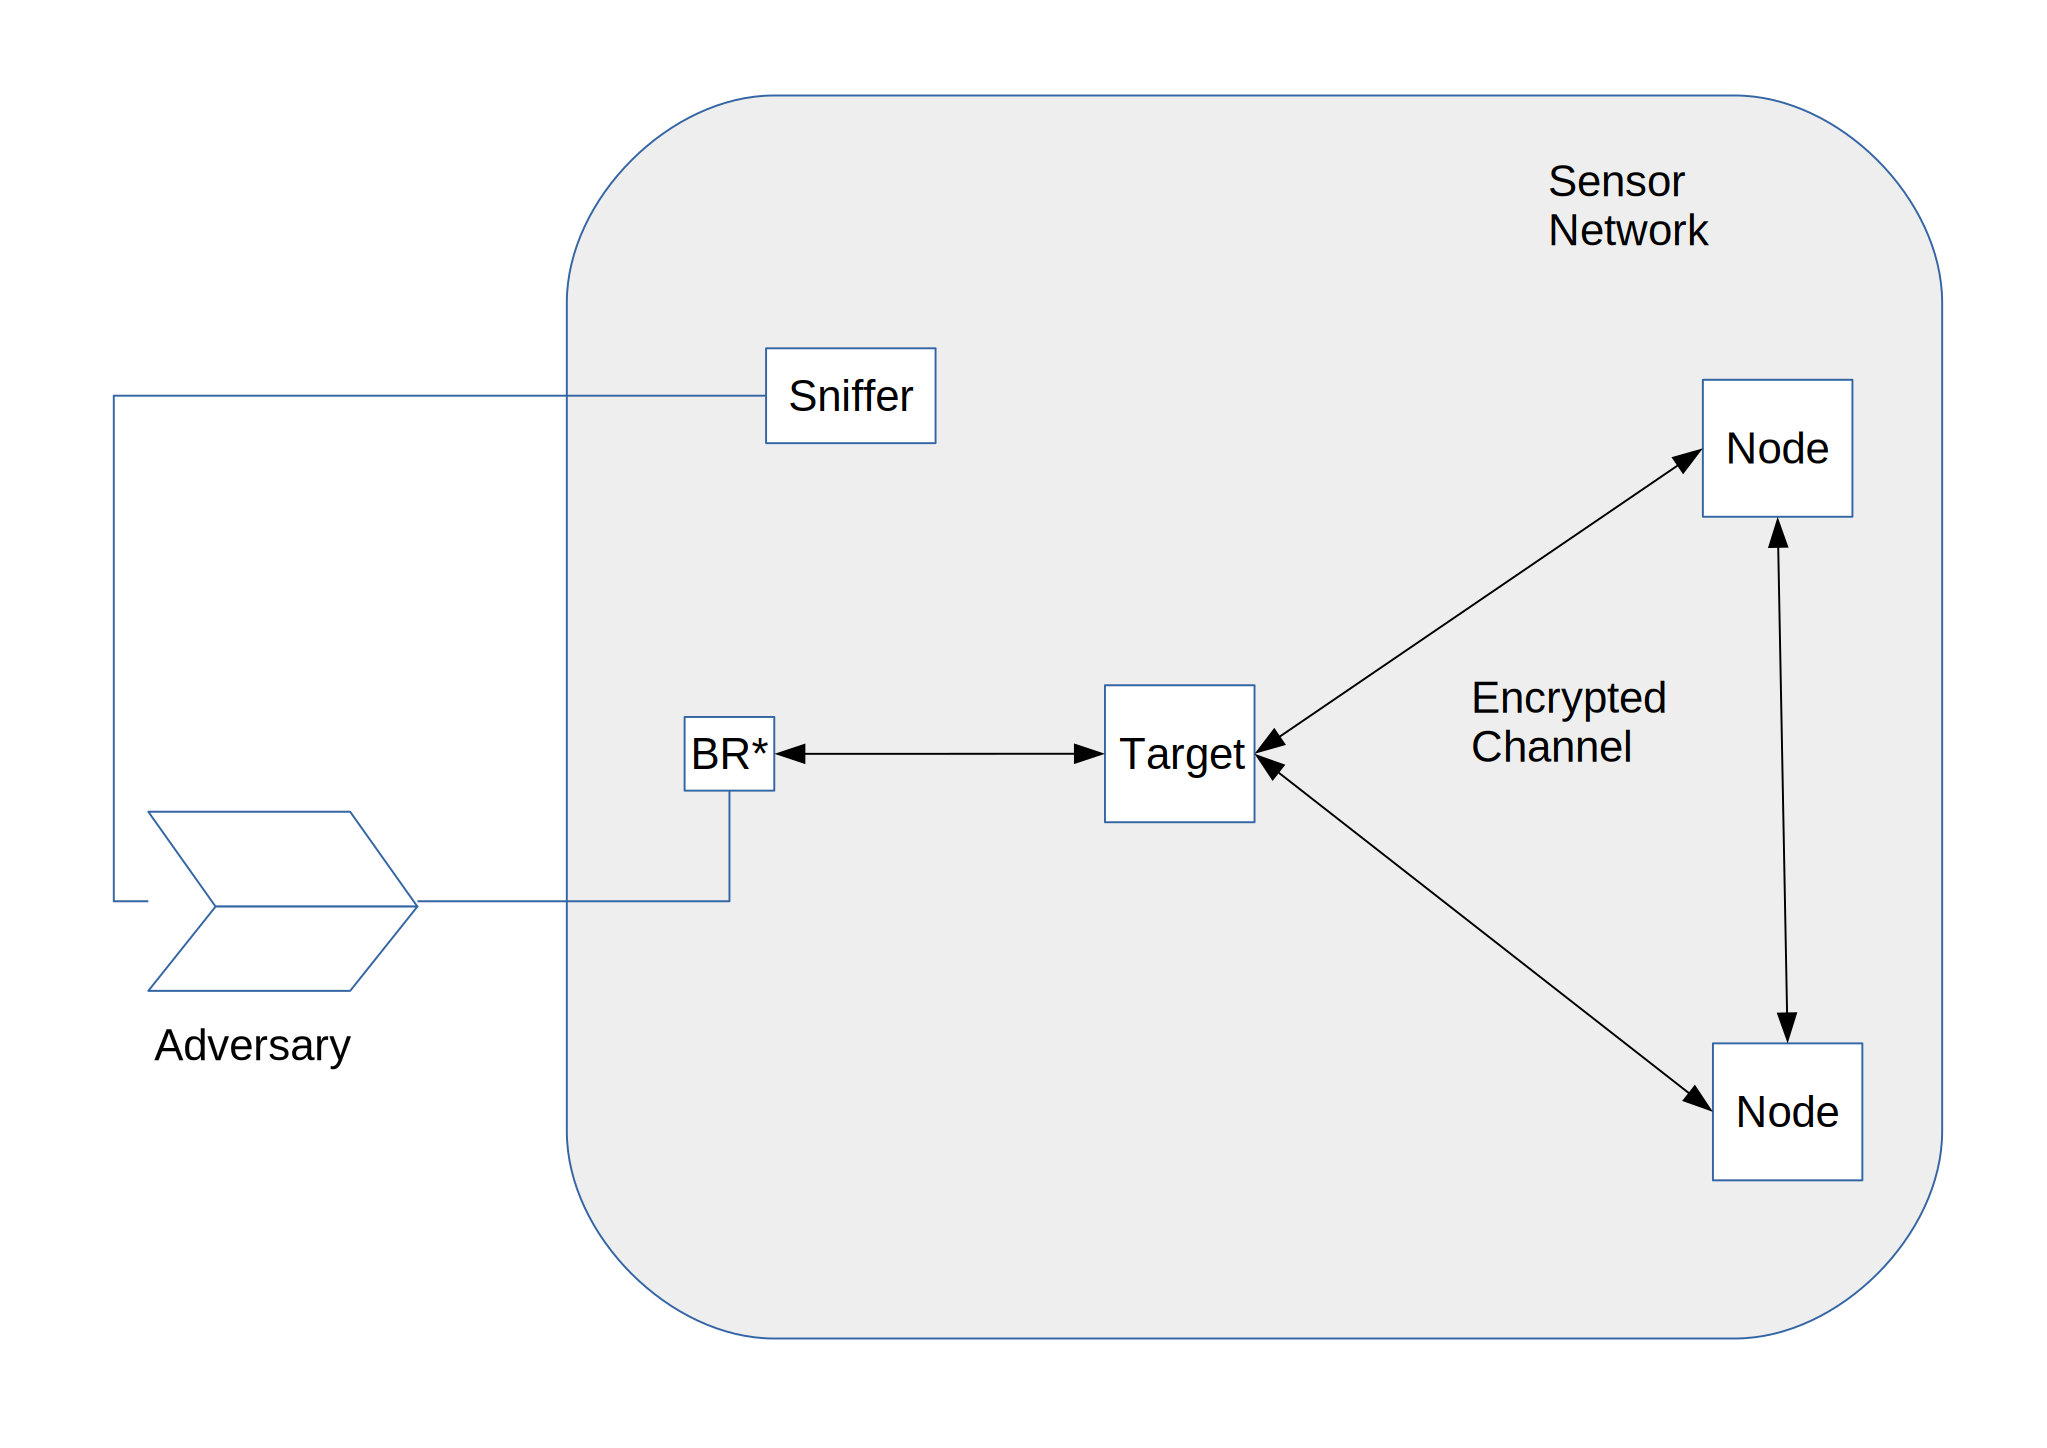
\includegraphics[width=0.9\textwidth,]{fig/setup.png}
	\caption{Experiment Setup} \label{Fig: Experiment Setup}
\end{figure*}

\begin{description}[style=nextline]
	\item[Sensor Network]
	The greyed area on the right inside the rectangle of \Cref{Fig: Experiment Setup} represents a WSN application.  The topology is dynamic and can change due to the application.  We make no further assumptions about the exact application at this point for generality.
	
	\item[Sensor Node]
	Each Sensor Node is a device with support of the protocol suite described in \Cref{Tbl: Summary of WSN Building Blocks}. All Sensor Nodes are connected to the same 6LoWPAN network. We do not impose the use of CoAP in our setup; instead, we assume applications may directly use the interface of UDP( or DTLS). More details are  are given in the later sections.
	
	\item[Border Router]
	Border Router is a special instance of Sensor Node. In addition to RF, Border Routers are additionally connected to other devices via different connections. In the experiments of this project, Border Routers are connected to a laptop through a USB connection. Border Router bridges two network. In the scenario of \Cref{Fig: Experiment Setup}, the Border Router is used to transmit IPv6 packets sent from the laptop. From a perspective of other Sensor Nodes in the WSN, a Border Router appears no different to the others. In many real world applications, the Border Router is connected to a management machine and serves as the DODAG root but this is not necessary in this experiment.
	
	\item[Sniffer]
	Sniffer is another special instance of Sensor Node. The Sniffer passively captures all frames it receives and does not transmit anything at all; thus it is transparent to other Sensor Nodes in the network. In our setup as of \Cref{Fig: Experiment Setup}, the Sniffer pipes any frames it captured to the Laptop. From a practical perspective, the hardware device of a Sniffer has a limited effective radius and thus would not be able to capture all frames in WSNs of wide deployment; however this can be easily overcame by deploying multiple synchronised Sniffers to cover a wide area. In our experiments, we assume every frame in the network is captured by the Sniffer.
	
	\item[Laptop]
	The Laptop in our experiment represents an adversary with unequally supreme resources comparing to the Sensor Nodes in terms of energy, memory and computational power. In our setup of \Cref{Fig: Experiment Setup}, the Laptop, which also represents the adversary, has access to all traffic captured by the Sniffer and is allowed to interact with other Sensor Nodes through the Border Router if authentication is not required to join the network.
\end{description}

\section{Operating System}

We use Contiki\cite{Contiki} to build our experiments.  Our source code are tested  with the release version of Contiki 3.0 which is available at:

\begin{center}
	\url{https://github.com/contiki-os/contiki/releases/tag/3.0}.
\end{center}

\subsection{Brief Introduction to Contiki:}

The official instruction for using Contiki is available at:
\begin{center}
	\url{http://www.contiki-os.org/start.html}
\end{center}

Contiki is an open source embedded system crafted for IoT devices. It has a good support on many recent hardware and it is optimised for code size. Comparing to Operating Systems for PCs, Contiki does not provide a User Interface, UI. Instead, the embedded system provides a framework for developers to use C language to write (mostly) hardware portable codes, as well as a set of APIs including clock library, simple process management and network interfaces,etc.

To use Contiki, there are basically three steps:

\begin{enumerate}
	\item Write the application code in C. There are plenty of code in the Contiki example folder that can be used as frameworks.
	\item Compile the source code according to the target device through \textit{make} command. Note that the root of Contiki source code must be correctly specified in the \textit{makefile}.
	\item Upload (also called ``burn'') the binary code to your device. 
\end{enumerate}

The application code is automatically executed whenever the device is powered on.

\section{Devices}

Three models of device are adopted in this project:

\begin{itemize}
	\item \textbf{TelosB}\cite{TelosB}, as known as Sky mote. This is a popular model for WSNs featuring low cost. As a trade off, TelosB has only very constrained performance in terms of bandwidth, available code size and processing power.
	
	\item \textbf{CC2538}\cite{CC2538}. This is a relatively powerful model with an ARM-Cortex M3 processor. To our knowledge, this is one of the becoming dominant device used in WSN applications.
	
	\item \textbf{Wismote}\cite{Wismote}. This model is used as a performance upgraded version of TelosB in this project. In this project, Wismote \textbf{IS ONLY USED IN SIMULATIONS}. 
\end{itemize}

All these nodes are 802.15.4\cite{802154} compatible and does not have any sensor attached by default. We omit further hardware details as it is beyond the scope of this project. 

\subsection{Cooja Simulator}

The Contiki source code includes the Cooja simulator under its tools folder. The official instruction of using the Cooja simulator is available at 

\begin{center}
	\url{http://www.contiki-os.org/start.html}
\end{center}

Cooja provides simulation for a whole WSN application. It generates simulation data for serial output, LED status and radio traffic. An example of Cooja execution is shown in \Cref{Fig: An Example of Cooja Execution}.

\begin{figure*}[h!]
	\center
	\includegraphics[width=0.8\textwidth]{fig/cooja_example.png}
	\caption{An Example of Cooja Execution}
	\label{Fig: An Example of Cooja Execution}
\end{figure*}

\Cref{Fig: An Example of Cooja Execution} shows a simulation simulating the exact same WSN topology as described in \Cref{Fig: Experiment Setup}, with \textcircled{1} being the Border Router. 

In this project, we are mostly interested into the radio traffic, captured by the ``Radio messages'' plug in which acts as the Sniffer in \Cref{Fig: Experiment Setup}. The corresponding pcap file is written by Cooja alongside the simulation under ``cooja/build/'' folder, which can later be opened by Wireshark\cite{Wireshark} for analysis, as shown in \Cref{Fig: A Wireshark Example}.

\begin{figure*}[h!]
	\center
	\includegraphics[width=0.8\textwidth]{fig/wireshark_example.png}
	\caption{A Wireshark Example}
	\label{Fig: A Wireshark Example}
\end{figure*}

As of the time of writing this report, Cooja in Contiki release 3.0 supports simulation for TelosB and Wismote. CC2538 is not yet supported by the current version.

\section{Security Protocols}
\subsection{LLSEC}

\subsection{DTLS}

\section{Applications}


%\begin{itemize}
%\item{\bf Adversary} is a malicious party that tries to illegally reveal information from the encrypted traffic.
%\item{\bf Border Router}, or BR, is a device that connects adversary to the sensor network. \textbf{BR is not allowed when LLSEC is enabled} as the adversary does not have the key and hence cannot connect into the network. We will discuss more about LLSEC in \Cref{Chp: LLSEC}.
%\item{\bf Sniffer} passively captures all traffic in the network. 
%\item{\bf Target} and {\bf Nodes} are sensors deployed in the sensor network. They communicates to each other through encrypted channels.
%\item{\bf Sensor Network} discussed in this paper is a 6LowPAN network based on Contiki OS.
%\end{itemize}

%Realistically speaking, this scenario could happen say an adversary sitting near a smart house with a laptop attached to a SoC\footnote{System on Chip} device, or your malicious neighbour walks into your smart house with her smart phone.
%
%\section{Adversary Power}
%The powers assumed in the experiments are considered to be practical in real life.
%
%When LLSEC is enabled, all traffic, including RPL\footnote{Routing Procol for Low-power and Lossy Networks} messages, are encrypted; therefore no external nodes can connect to the network as an external node cannot send any valid RPL messages to join the network. The adversary only passively sniffs all traffic.
%
%With LLSEC disabled, the adversary can therefore join the sensor network through a BR and hence is also capable to send messages to the target(s). However, she will not be able to inject any message into an encrypted channel such as a DTLS channel.
%
%\section{Types of Packets}
%We simply categorise the packets into two types:
%\begin{itemize}
%\item {\bf Network Management Packets}: These are the packets generated by the protocols to  maintain the functionality of network, such as MAC ACKs, RPL messages or ICMP messages.
%\item {\bf Data Packets}: These are those packets generated by applications running on sensor nodes., such as a CoAP packet.
%\end{itemize}
%
%This is only a subjective rough categorisation and may not be precise. For example an TCP data packet may set its ACK flag, or DTLS handshake packets could ambiguously fall into both categories. However, we ignore this ambiguity as it is not our focus.
\chapter{Link Layer Security: noncoresec} \label{Chp: LLSEC}

In this chapter, we provide an analysis for the Link Layer security measure noncoresec, which we have explained in \Cref{Subsec: 802.15.4 Security Implementation in Contiki}.

\section{Protocol and Implementation}
%Reset Problem
In this section, we analysis the noncoresec implementation with respect to the problems described by \cite{802154sec}. 

\subsection{Nonce Reuse}

As we have explained in \Cref{Subsec: 802154 Nonce}, the only variable field in the nonce is Frame Counter. Since noncoresec only supports network shared key, there are two potential problems according to \cite{802154sec}, namely nonce reuse and anti replay. Further inspecting the source code, we realised that the counter is declared as a static value and is initialised to $0$ on each reboot.

Our experiments confirmed the vulnerability. We simulated two executions of  broadcast\_example of keyllsec in \Cref{Sec: Applications}, broadcasting the same message. Our data\cite{NonceReuseData} showed that frames with the same Frame Counter results into the same ciphertext. In reality, this vulnerability implies that an adversary capable to reset the device can eventually learn the difference in plaintext by calculating the difference of ciphertext with the same Frame Counter, causing severe breach of data confidentiality.

One solution might be to store part of the Frame Counter on the flash and increases that value on each time reboot. Assume the device averagely sends one frame every minute stores the highest byte of Frame Counter, it is resilient in $2^8$ reboots and the lower bytes still has the space of $2^{24}$ frames, which holds up to nearly 32 years. Another solution could be to set the higher bytes of Frame Counter to a random value on each reboot. For example, by setting the highest byte to a uniformly distributed random value in $[0,255]$, the adversary is expected to successfully reset the Frame Counter to a specific value with probability of $2^{-8}$ on each reboot.

\subsection{Anti Replay}

\cite{802154sec} has pointed out that anti replay in 802.15.4 Security is incompatible with network key as the same ACL entry is shared among multiple nodes, causing confusion of Replay Counter in ACL. However, with an inspection of the source code of Contiki, we realised that the noncoresec does not suffer the same problem as the ACL is not implemented; instead, a similar data structure is added to the routing table in kernel  associated to each source address.

\section{Common Analysis}

%Packet Length

%Timing for encryption

%RPL Messages

%Sequence Numbers

\section{Application Analysis}




%
%Link Layer Security, or LLSEC, is a security measure that implements cryptography at Data Link Layer\footnote{https://en.wikipedia.org/wiki/OSI\_model} which is only above Physical Layer.
%
%Introducing cryptography at a lower level has several benefits. Firstly, more data being encrypted reduces the observable packet features to an adversary, such as SRC\footnote{Source Address} and DST\footnote{Destination Address} field in the IP header which are very likely to be exploited by an adversary. Secondly, authentication at lower level also prevents an active adversary from joining the network which therefore weakens her power. 
%
%On the other hand, imposing cryptography at a lower level also brings more challenge to the design of sensor network architecture. The first problem is its overhead. For example, even for a node that only forwards a packet to its next hop, it must decrypt the whole packet to extract its routing information, and then re-encrypt it before transmission. This is particularly problematic in a mesh wireless sensor network as it could potentially downgrades the performance and causing energy consumption problems. More over, key management is also challenging due to the constrained computational power and power optimised lossy nature of wireless sensor network.
%
%It is noticeable that some packet features are not hidden even with LLSEC enabled, such as packet length, timing information and part of the MAC header in a 802.15.4 packet.
%
%\section{802.15.4 Security: {\it noncoresec}} \label{sec: noncoresec}
%{\it noncoresec}\cite{LLSEC} is the current implementation of LLSEC in Contiki. It implements AES\_CCM\_16 ciphersuite in 802.15.4 standard. This section briefly describes how it works.
%
%\begin{itemize}
%\item {\bf Key Management}: All nodes share a network wide AES key for both encryption and authentication. The key is hardcoded during the setup stage.
%
%\item{\bf AEAD\footnote{Authenticated Encryption with Associated Data}}: {\it noncoresec} implements AES\_CCM\_16 \footnote{CCM mode of AES-128 with 16 bytes MAC} as described in 802.15.4\cite{802154} which turns AES into a stream cipher. The same key is used for both encryption and authentication.
%
%\item{\bf Initial Vector (IV, or nonce)}: The IV for each packet is constructed from certain fields of unencrypted MAC header and therefore is public.
%\end{itemize}
%
%An adversary without the knowledge cannot join the sensor network protected by \textit{noncoresec} as she cannot sent out a valid RPL message.
%
%\section{Weak IV}
%
%\begin{figure}
%\centering
%\begin{tabular}{| l | l | l | l | l |}
%\hline
%Flags(1) & Addresses(8) & Frame Counter(4) & Security Level(1) & Block Counter(2)       \\ \hline
%\end{tabular}
%\caption{IV of 802.15.4 Frame with Security} \label{Tbl: 802154 Frame}
%\end{figure}
%
%One problem within the {\it noncoresec} implementation is the low variance of IV. The IV is a $16$ byte bit-string constitutes of the following fields(\Cref{Tbl: 802154 Frame}):
%\begin{itemize}
%\item {\bf Flags (1 byte)}: This field contains part of the MAC header. It is identical to most (basically all) of the data packets.
%
%\item{\bf Source Address (8 bytes)}: This is mapped from the source address field of the packet.
%
%\item{\bf Frame Counter (4 bytes)}: This field increases by 1 from 0 for each packet sent to prevent replay attack.
%
%\item{\bf Security Level (1 byte)}: This field indicates which ciphersuite to be used for this packet. In the case of AES\_CCM\_16, this is constantly 0x7.
%
%\item{\bf Block Counter (2 bytes)}: This field begins from 0x0 and increases by 0x1 for each block in CCM mode. The block length for AES-128 is 16 bytes. The 2 bytes counter is usually sufficient as it supports up to $2^{32}$ bytes of data whereas the minimum MTU\footnote{Maximum Transmit Unit, simply speaking this is the maximum length of a packet.} required by 6lowPAN standard\cite{rfc4944} is $127$ bytes.
%\end{itemize}
%
%In the current {\it noncresec} implementation, \textbf{Flags} and \textbf{Security Level} are constant. \textbf{Block Counter} always begins from 0x0 and the \textbf{Source Address} is also constant for a specific device. Such design leaves the 4 bytes \textbf{Frame Counter} the only field that is variable. This indicates that only $2^{32}$ messages are allowed without a collision of IV which is cryptographically considered to be inappropriate.
%
%\subsection{Reset Problem}
%The low variance of IV leads to a plaintext leakage problem which only requires the adversary to reboot the target node. 
%
%The idea is that rebooting the device resets the \textbf{Frame Counter} to 0x0; hence once a pair of packets with same \textbf{Frame Counter} is found, the difference of their plaintext can be computed by their ciphertext:
%\begin{equation*}
%\Delta p = c_1 \oplus c_2
%\end{equation*}
%where $\Delta p$ is the difference of plaintexts. $c_1$ and $c_2$ are their ciphertext respectively.
%
%\begin{example}
%\begin{figure*}
%\centering
%{
%	\includegraphics[width=0.9\textwidth,]{fig/resetproblem.png} 
%}
%\caption{Captured packets with {\it noncoresec} enabled} \label{Fig: reset problem}
%\end{figure*}
%
%\Cref{Fig: reset problem} demonstrates some packet captured\footnote{The duplicated packets are caused by the retransmission of ContikiMAC\cite{ContikiMAC}.} with {\it noncoresec} enabled. These packets are captured with a sensor broadcasting a 4 byte integer with left side of \Cref{Fig: reset problem} being $[00000000]_{16}$ and right $[12345678]_{16}$. Marked are the corresponding ciphertexts which are $[00127401]_{16}$ and $[12262279]_{16}$ respectively.
%
%As we can see, the difference of ciphertext is exactly the difference of plaintext:
%\begin{equation}
%\Delta p = [00127401]_{16} \oplus [12262269]_{16} = [12345678]_{16}
%\end{equation}
%\end{example}
%
%\section{Distinctive Packet Length for RPL Packets}
%Some RPL packets are shorter than the minimum length of data packets which can be used to distinguish the packets. Further more, some RPL packets set MAC header flags differently from data packets.
%
%\section{Performance Issue}
%The header overhead with LLSEC enabled is 20 bytes which is relatively a large overhead comparing to the 127 bytes MTU requirement of 6LowPAN standard\cite{rfc4944}.
\chapter{DTLS}



\section{Conflicting MTU between DTLS and 6lowPAN}
The abandoned CoDTLS.
\section{Overloading DTLS with LLSEC}
\chapter{Application Detection}
Similar to website fingerprinting, we try to identify the application running on target note by its traffic. This chapter discusses some general idea without a specific application.

\section{Network Protocol Headers}
Since most information in MAC\footnote{Media Access Control, not to be confused with the cryptographic term Message Authenticate Code.}, IP and UDP headers are related to routing and network maintenance and thus independent except the length fields and CRC\footnote{Cyclic Redundancy Check, a code to detect or correct transmission error}. 

\section{Packet Length}
Packet length is usually the most interested target in traffic analysis. However, packet lengths are also highly application dependant; thus we are not pursuing this topic further without a specific application.

\section{Timing Packet Response}
Unlike web applications where the client and server are usually physically distant, sensor networks can sometimes located in a concentrated area, such as a house which its radius can be less than 10 meters. 

These features theoretically enables one to capture all traffics in such a sensor network. As opposed to the case of Internet where packets are usually timed on the client’s side and thus network latency (RTT\footnote{Round-Trip Time}) must be concerned, being able to capture all traffic in the network provides  much more accurate timing information and hence may be exploited to develop more efficient attacks.

\begin{definition}
In a Request-Response application model, \textbf{RI}, {\bf Response Interval}, is defined as the interval between a request packet being received and its response being sent.
\end{definition}

\begin{example}
\begin{figure}
\centering
{
	\includegraphics[width=\textwidth,]{fig/responsetime.png}
}
\caption{Capture of a ping packet}
\label{fig: ping packet}
\end{figure}

\begin{table}[!]
\centering
\begin{tabular}{|l|l|l|l|l|}
\hline
Time (ms) & From (ID) & To (ID) & Length (bytes) & Type          \\ \hline
1961218   & 1         & 2       & 108            & ICMP ECHO \\ \hline
1961222   & 2         & 1       & 5              & 802.15.4 ACK  \\ \hline
1961230   & 2         & 1       & 107            & ICMP ECHO \\ \hline
\end{tabular}
\caption{Packet Features of an ICMP ECHO request and response}
\label{Tbl: ping}
\end{table}

Three packets are marked out in \Cref{fig: ping packet} which forms an instance of ICMP ECHO\cite{rfc1122} (also known as PING) session. The extracted packet features are displayed in \Cref{Tbl: ping}.

\begin{description}
\item[Explanation of the Packets:]\hfill \\
The first packet is an ICMP ECHO request and the third packet being its response. The second packet is a 802.15.4 ACK\footnote{This is an acknowledgement from the receiver that notifies the sender that the packet has been received.} and is thus transparent to the upper ICMP protocol.
\end{description}

From this example we can see that the RI for this PING session is:
\begin{equation*}
1961230 - 1961218 = 12 \text{(ms)}
\end{equation*}

\end{example}

Timing information can be exploited by several attacks, such as \cite{Peekaboo} and \cite{rsatiming}.

We have experimentally measured a RNG\footnote{Random Number Generator} call on Wismote platform in the Cooja simulator is roughly 0.3 ms.

\section{PINGLOAD: PING side-channel for Payload }
Support of ICMP ECHO is required by \cite{rfc1122} and is also enabled in Contiki OS by default. However, our experimental results shows that the response time of these ping packets could potentially be exploited to reveal the application running on target sensor node.

We call such technique {\bf  Application Fingerprinting}.

\subsection{Hypothesis}
A phenomenon we realised is that when a ping packet arrived while the target node is executing some payload, say reading a sensor or processing data, the PING RI begins to vary comparing to a stable value  when no there is no payload. 

\begin{example}
\begin{figure}
\centering
{
  \includegraphics[width=1\textwidth]{fig/pingri.png}
}
\caption{An example of PING RIs with different payload}
\label{Fig: PINGLOAD RIs}
\end{figure}
\Cref{Fig: PINGLOAD RIs} shows RIs of PING collected in two experiments. The upper half are collected with the target is constantly sleep whilst the lower half occasionally receives a request which triggers the target to call RNG. We can see that the PING RI varies alongside the target is given some payload from this figure.
\end{example}

The data shown in \Cref{Fig: PINGLOAD RIs} suggests that the “plain”, that is without any interference, PING RI is 12 to 13 ms. Further more, those variations of  PING RI is very likely caused by the payload of the target.

This experiment inspired that the distributions of PING RIs might vary according to the payload of target and could possibly considered as an fingerprint of the target’s application. In other word, an adversary could possibly tell whether the target is running a specific application by looking at its PING RIs distribution.

The attack is strait forward:
\begin{description}
\item[Profile sleep RIs]: \hfill\\
The PING RIs for a sleeping node of the same platform can be profiled by pinging a sleeping node. We denote the sleeping profile as $RI_{sleep}$. 

\item[Fingerprint application]: \hfill\\
The adversary collects PING RIs on a profiling node with known application. The profiling node needs to be of the same platform and executing the same code of the target’s. The application fingerprint denotes as: $F_p=\{p_1, p_2, ... , p_n\}$. 

\item[Collect fingerprint of target]: \hfill\\
The adversary then collects the PING RI for the target node by pinging it. We denote the collected data as: $F_t=\{t_1, t_2, ..., t_m\}$.

\item[Extract Featured RIs]: We can remove them from the data sets and keep the PING RIs those has been interfered by the application. We denote the extracted RIs as \textbf{Featured RIs}:
\begin{eqnarray*}
F’_p = \{x | x \in F_p,  x \notin RI_{sleep}\}\\
F’_p = \{x | x \in F_t,  x \notin RI_{sleep}\}
\end{eqnarray*}

Practically speaking, the PING protocol are designed to be responded immediately for diagnosis purpose; hence $RI_{sleep}$ usually has an extremely low variance and its mean is also much less than $F_p$ and $F_t$.

Using the Featured RIs not only provides a better vision of the fingerprint but also removes the error caused by different frequency of the target code being executed, as all the Featured RIs are actually collected when the node is at a non-sleeping state. 

\item[Estimate Distribution (Optional)]: \hfill\\
We then estimate the distributions of $F’_p$ and $F’_t$, denote as $D_p$ and $D_t$. A naive method is to simply use their histograms. An example of such histograms are shown as \Cref{Fig: featuredri_rng}.

\begin{figure}
\center
{
	\includegraphics[width=0.49 \textwidth]{fig/featuredri_rng1.png}
	\includegraphics[width=0.49 \textwidth]{fig/featuredri_rng2.png}
}
\caption{Two examples of RNG’s Featured RIs histogram}
\label{Fig: featuredri_rng}
\end{figure}

\item[Distinguish Distributions]: \hfill\\
Finally we test whether $D_t$ and $D_p$ are the same distribution. An naive way is to compute the correlation of counts of the histograms. We conclude the target node is running the profiled application if $D_t$ and $D_p$ are the same distribution.
\end{description}

Practically speaking, the key point of Application Fingerprinting is to test whether the target’s Featured RIs, i.e. $F’_t$, is sampled from same distribution of the profiled one, i.e. $F’_p$; therefore estimating their distribution might not be necessary for some statistical methods such as t-tests. However as we can see in \Cref{Fig: featuredri_rng}, PING RIs’ distribution are very unlikely to be normalised. Therefore a future work is to find a better distinguishing method than the current naive one.

\subsection{Experiment Result}
We tried our Application Fingerprinting method above on a Cooja simulated Wismote platform with different code. \textbf{In conclusion, the fingerprint appears to be effective for certain circumstances but will tends to result into false positives as the profiled application and target application gets similar to each other.}

To be more specifically, the target node execute some specific code upon receiving an application layer protocol request, similar to CoAP. Further more, all traffic are protected by DTLS with TLS\_PSK\_WITH\_AES\_128\_CCM\_8 ciphersuite. Both intervals of PINGs and the application request are set to some asynchronised value to avoid overflooding the target and to create a ‘more realistic’ simulation.

Everything other than the examined code are the same for all experiments. Two samples are collected independently for each code to simulate a fingerprinting scenario. The histograms are clustered by 5ms.

We examined two classes of codes:
\begin{description}
\item[RNG Calls]: \hfill\\
The target node repeatedly calls RNG for $i$ times. We examined their Featured PING RI for different values of $i$. The reason for picking RNG is that on some platforms where a hardware RNG is provided, the call to it is expected to be similar to a call to a sensor reading which is actually an interrupt. Results are shown in \Cref{Tbl: pingload RNG}.

\item[Arithmetic Operations]: \hfill\\
The target node repeatedly does arithmetic operations, namely addition, multiplication and modular, on two random generated word size integers for 10000 times. This class is particularly interested from a cryptographic point of view as the number of arithmetic operations could potentially developed to key recovering attacks. Results are shown in \Cref{Tbl: pingload arth}.
\end{description}



\begin{table}
\centering
\begin{tabular}{|c|cccc}
\hline
\textit{\textbf{Correlations}} & \multicolumn{1}{c|}{i=50} & \multicolumn{1}{c|}{i=100} & \multicolumn{1}{c|}{i=2500} & \multicolumn{1}{c|}{i=5000} \\ \hline
i=50                           & \textbf{0.988}            & 0.891                      & -0.014                      & -0.033                      \\ \cline{1-1}
i=100                          & 0.891                     & \textbf{0.973}             & -0.025                      & -0.042                      \\ \cline{1-1}
i=2500                         & -0.014                    & -0.025                     & \textbf{0.993}              & -0.035                      \\ \cline{1-1}
i=5000                         & -0.033                    & -0.042                     & -0.035                      & \textbf{0.985}              \\ \cline{1-1}
\end{tabular}
\caption{Correlations for RNG}
\label{Tbl: pingload RNG}
\end{table}

\begin{table}
\centering
\begin{tabular}{|c|ccc}
\hline
\textit{\textbf{Correlations}} & \multicolumn{1}{c|}{+} & \multicolumn{1}{c|}{*} & \multicolumn{1}{c|}{\%} \\ \hline
+                              & \textbf{0.990}         & \textbf{0.990}         & \textbf{0.988}          \\ \cline{1-1}
*                              & \textbf{0.990}         & \textbf{0.989}         & \textbf{0.985}          \\ \cline{1-1}
\%                             & \textbf{0.988}         & \textbf{0.985}         & \textbf{0.984}          \\ \cline{1-1}
\end{tabular}
\caption{Correlations for word arithmetic operations}
\label{Tbl: pingload arth}
\end{table}

\begin{table}[]
\centering
\begin{tabular}{|c|c|}
\hline
\textbf{\textit {Correlations}} & +     \\ \hline
i=50         & 0.877 \\ \hline
\end{tabular}
\caption{Correlation for $i=50$ and addition}
\label{Tbl: pingload rng arth}
\end{table}

We also computed the correlation for $i=50$ and addition, as shown in \Cref{Tbl: pingload rng arth}.

The results suggests the following conjectures:
\begin{enumerate}
\item The results for RNG suggests that the fingerprinting is effective for this class of code, as the same code results into nearly perfect correlations ($\geq 0.95$).

\item Even relatively slight changes can be detected, as we can see the correlation dropped to $0.891$ alongside 50 iterations of RNG calls (50 RNG calls take about 1.4ms).

\item The results for arithmetic operations indicates that their  fingerprint are unlikely to be distinguishable. There are two potential causes we have considered:
\begin{enumerate}
\item The differences between these operations are too small to be detected.

\item Experiment methodology error. Since the target node we used during the experiments call RNG twice upon each request to generate two operands whilst the word arithmetic operations have much lighter weigh comparing to RNG at magnitude level; thus the fingerprint is dominated by RNG rather than word arithmetic operations. As a result, we can see that a relatively high correlation can be observed between word addition and 50 RNG calls as shown in \Cref{Tbl: pingload rng arth}.
\end{enumerate}
\end{enumerate}

\subsection{General Hypothetical Model}
THE BLACK BOX MODEL
\section{Conclusion}
In this paper we presented a study on the RNG design of CC2538. First, we revised the problem that using a 16 bit LFSR as PRNG is a bad idea and demonstrated how this design flaw can be exploited to break DTLS running on these devices. Secondly we presented a study to its seeding method and showed how such it could be remotely tampered by an adversary sending jamming signal to the device.

In fact the same RNG design has also been adopted many other products in the CC series including CC2420\cite{CC2420Manual}, CC2430\cite{CC2430Manual}, CC2520\cite{CC2520Manual} and CC253X, CC2540/41 series\cite{CC2530Manual}. We imagine all these products suffer the same problems. Fortunately the latest CC26XX/CC13XX\cite{CC26XXManual} has abandoned this design and implemented a dedicated RNG which TI describes as: (Chapter 16 in CC26XX/CC13XX Manual\cite{CC26XXManual})
\begin{quote}
The true random number generator (TRNG) module provides a true, nondeterministic noise source for the
purpose of generating keys, initialization vectors (IVs), and other random number requirements. The
TRNG is built on 24 ring oscillators that create unpredictable output to feed a complex nonlinear
combinatorial circuit. That post-processing of the output data is required to obtain cryptographically secure
random data.
\end{quote}

We sincerely hope this TRNG will provide the future IoT applications a secure RNG.

\section{Acknowledgement}
We have many thanks to (alphabetically) George Oikonomou for providing us much help in Contiki OS and the OpenMote devices, Geoff Hilton who helped us on RF designs and Jake Longo Galea who offered many signal processing advises.
\appendix
\chapter{Formal Proof of \Cref{Te: IR}} \label{Prf: IR}
\begin{proof}
	%Independent random variables does not leak.
	Since $X$ and $Y$ are independent, therefore
	\begin{eqnarray*}
		\begin{aligned}
			P(x,y) &= P(x)P(y) \\
			P(x|y) &= P(x)
		\end{aligned}
	\end{eqnarray*}
	where $x \in X$ and $y \in Y$.

	For Mutual Information and Capacity, we have:
	\begin{eqnarray*}
		\begin{aligned}
			H(X|Y) 
			&= - \sum_{x \in X} \sum_{y \in Y} P(x,y)\log{P(x|y)} \\
			&= - \sum_{x \in X} \sum_{y \in Y} P(x)P(y)\log{P(x)} \\
			&= \sum_{y \in Y} P(y) (- \sum_{x \in X}P(x)\log{P(x)}) \\
			&= \sum_{y \in Y} P(y) H(X) = H(X) \sum_{y \in Y}{P(y)} \\
			&= H(X)
		\end{aligned}
	\end{eqnarray*}
	
	Therefore
	\begin{eqnarray*}
		\begin{aligned}
			I(X;Y) &= H(X) - H(X|Y) = H(X) - H(X) = 0 \\
			C &= \sup_{\forall P(X)} I(X;Y) = \sup_{\forall P(X)} 0 = 0
		\end{aligned}
	\end{eqnarray*}
	
	Similarly for gain function based leakage\cite{GLeakage},
	\begin{eqnarray*}
		\begin{aligned}
			V_{g}(\pi, C) 
			&= \sum_{y \in Y}{\max_{w \in W}\sum_{x \in X}{\pi[x]C[x,y]g(w,x)}} \\
			&= \sum_{y \in Y}{\max_{w \in W}\sum_{x \in X}{\pi[x]P(y|x)g(w,x)}} \\
			&= \sum_{y \in Y}{\max_{w \in W}\sum_{x \in X}{\pi[x]P(y)g(w,x)}} \\
			&= \sum_{y \in Y}p(y){\max_{w \in W}\sum_{x \in X}{\pi[x]g(w,x)}} \\
			&= \max_{w \in W}\sum_{x \in X}{\pi[x]g(w,x)} = V_{g}(\pi)
		\end{aligned}
	\end{eqnarray*}
	
	Therefore
	\begin{equation*}
		H_g(\pi, C) = -\log{V_g(\pi, C)} = -\log{V_g(\pi)} = H_g(\pi)
	\end{equation*}
	
	Hence 
	\begin{eqnarray*}
		\begin{aligned}
			L_g(\pi, C) &= H_g(\pi) - H_g(\pi,C) = H_g(\pi) - H_g(\pi) = 0\\
			ML_g(C) &= \sup_{\pi} L_g(\pi, C) = \sup_{\pi} 0 = 0
		\end{aligned}
	\end{eqnarray*}
\end{proof}



\chapter{Details of Packet Feature Cross Reference} \label{Detail Cross Reference}

For the exploited traffic features in 

\begin{description}[style=nextline]
	\item[Direction]
	In our applications, the directions of packet is a predictable constant. We consider this is not a 
	
	\item[Length]
	The is effectively the packet size in implicit observables.
	
	\item[Frequency Distribution of Length]
	The same feature can be computed by packet sizes. However, since there are typically only two packets in a trace, the result is $0.5$ for the length of Request packet and $0.5$ for the length of Response packet. In a one packet Session there is only one value in the distribution with probability of $1$. This feature is applicable but with extremely low entropy of $1$ or $0$.
	
	\item[Size, HTML and Number Markers]
	In a two packet Session there is only one direction change in a trace; thus the markers constantly mark the second packet. In an one packet Session this feature is not applicable.
	
	\item[Total Bytes]
	The same feature can be computed through packet sizes.
	
	\item[Percentage Incoming Packets]
	The term ``incoming'' refers to the direction of web server to the browser in its original Web Fingerprint literature. In our experiments we assumed the adversary monitors all packets in the network; thus there is not an explicit definition of ``incoming'' and ``outgoing''. Even though we can similarly define ``incoming'' as from Sensor Node to Manager, this is feature is fixed given an application. This value is constantly $50\%$ for a two packets Session and $100\%$ for a one packet Session.
	
	\item[Number of Packets]
	Since UDP does not segment any application data, the number of packets in a trace is a constant given an application. 
	
	\item[Total Time]
	In a two packets Session this is exactly the interval between Request and Response. In an one packet session this is not applicable.
	
	\item[Total Per-direction Bandwidth]
	Since there is at most only one packet at each direction, this feature is effectively a single packet size divided by total time for each direction.
	
	\item[Traffic Burst]
	Traffic burst is reduced to packet size in our applications as there is at most only one packet each direction.
\end{description}

Notice that we ignored Traffic Bursts since it is reduced to packet length in our applications as explained above.

According to \Cref{Cor: Constant Leakage}, features with constant value are non leakable features. 

\chapter{Leakage of Linear Packet Size} \label{Linear Leakage}

Modelling the leakage of packet length as a channel $C(l_{C},l_{P})$ as in other Information Theoretic approaches we described in \Cref{Subsec: Information Theory}, we have a deterministic channel such that:

\begin{equation}
	C(l_{P}, l_{C}) = P(l_{P} | l_{C}) = 
	\begin{cases}
		1 &\text{if: } l_{C} = l_{P} + b \\
		0 &\text{otherwise}
	\end{cases}
\end{equation}

and

\begin{equation}
	C^{-1}(l_{C}, l_{P}) = P(l_{C} | l_{P}) = 
	\begin{cases}
		1 &\text{if: } l_{C} = l_{P} + b \\
		0 &\text{otherwise}
	\end{cases}
\end{equation}

So

\begin{equation}
	P(l_{P} , l_{C}) = P(l_{P}) P(l_{C} | l_{P}) =
	\begin{cases}
		P(l_{P}) &\text{if: } l_{C} = l_{P} + b \\
		0 &\text{otherwise}
	\end{cases}
\end{equation}

Therefore\footnote{Information Theory defines $0\log{0} = 0$.},
\begin{equation}
	P(l_{P} , l_{C}) \log{P(l_{P} | l_{C})} = 
	\begin{cases}
		P(l_{P})\log{1} = 0 &\text{if: } l_{C} = l_{P} + b \\
		0 \log{0} = 0 &\text{otherwise}
	\end{cases}
\end{equation}

Hence
\begin{equation}
	H(L_{P} | L_{C}) = - \sum_{l_{C} \in L_{C}} \sum_{l_{P} \in L_{P}}P(l_{P} , l_{C}) \log{P(l_{P} | l_{C})} = - \sum_{l_{C} \in L_{C}} \sum_{l_{P} \in L_{P}} 0 = 0
\end{equation}
where $L_{P}$ and $L_{C}$ are the possible length in bytes of encrypted and unencrypted packets.

In this case, the Mutual Information is:
\begin{equation} \label{Eq: MI in length}
	I(L_{P};L_{C}) = H(L_{P}) - H(L_{P} | L_{C} ) = H(L_{P}) - 0 = H(L_{P})
\end{equation}

For the Capacity, according to \Cref{Eq: MI in length}, $I(L_{P};L_{C})$ has its maximum value when $L_{P}$ is uniformly distributed:
\begin{equation} \label{Eq: Cap in length}
	Capacity = \sup_{\forall L_{P}}{I(L_{P};L_{C})} = \sup_{\forall L_{P}}H(L_{P}) = - \sum_{i = 1}^{|L_{P}|}|L_{P}|^{-1}\log{|L_{P}|^{-1}} = \log{|L_{P}|}
\end{equation}

In another word, \Cref{Eq: MI in length} and \Cref{Eq: Cap in length}  imply that averagely all bits of $l_{P}$ is leaked through $l_{C}$.

For the gain function based leakage\cite{GLeakage}, we realised that it would be hard to quantify the leakage without a specific gain function. Therefore instead, we provide an analysis with min-leakage.

In this case, the Posterior Vulnerability is:
\begin{equation}
	\begin{aligned}
		V(\pi_{L_P}, C^{-1}) 
		&= \sum_{l_{C} \in L_{C}} \max_{l_{P} \in L_{P}} \pi_{L_P}[l_P]C^{-1}[l_P,l_C] \\
		&=  \sum_{l_{C} \in L_{C}} P(l_C) \max_{l_{P} \in L_{P}} P(l_P | l_C) \\
	      &= \sum_{l_{C} \in L_{C}} P(l_C) = 1 \\
	\end{aligned}
\end{equation}

Therefore
\begin{equation}
	\begin{aligned}
		H_{\infty}(\pi_{L_{P}}, C^{-1})
		 &= - \log{V(\pi_{L_{P}}, C^{-1})} = - \log1= 0
	\end{aligned}
\end{equation}

Thus the min-leakage is:
\begin{equation}
	\begin{aligned}
	L(\pi_{L_P}, C^{-1}) 
	 &= H_{\infty}(\pi_{L_P}) - H_{\infty}(\pi_{L_{P}}, C^{-1}) \\
	 &= H_{\infty}(\pi_{L_P}) - 0 \\
	 &= H_{\infty}(\pi_{L_P})
	\end{aligned}
\end{equation}

And finally:
\begin{equation}
	ML(C^{-1}) = \sup_{\pi_{L_P}}{L(\pi_{L_P},C^{-1})} =  \sup_{\pi_{L_P}} H_{\infty}(\pi_{L_P}) = \log{|L_P|}
\end{equation}

This result consists with our intuition and the Capacity in \Cref{Eq: Cap in length} that all bits of $l_P$ are leaked through $l_C$.


%\bibliographystyle{ieeetran}
%\bibliography{references,rfc}
\printbibliography

\end{document}
